% =====================================================================
% THIS FILE IS THE SOURCE. Edit it, then rebuild the PDF with:
%     bash tools/compile.sh Unit_07_Prediction_and_Its_Uncertainty
% (run from the Course_Rewrite folder; it compiles twice and reports
%  page count, overfull boxes, and em dashes)
%
% Do not edit the PDF directly. Figures are the fig_*.pdf files in this
% folder, regenerated by tools/make_module*_slide_figs.py.
%
% Originally converted from the 15-module draft by a one-shot script now
% parked in tools/one_shot_generators/. Re-running those would discard
% anything you change here, so they are kept out of tools/ on purpose.
% =====================================================================
\documentclass[aspectratio=169]{beamer}
\usetheme{default}
\usefonttheme{professionalfonts}
\usepackage{amsmath, amssymb, amsfonts}
\usepackage{graphicx}
\usepackage{booktabs}
\usepackage{bm}
\usepackage{hyperref}

\mode<presentation> {
    \usetheme{Frankfurt}
    \usecolortheme{default}
}

% == notation shortcuts ==
\newcommand{\xbar}{\bar{x}}
\newcommand{\yhat}{\hat{y}}

% Recurring motifs (color-coded).
\newenvironment{principle}[1]{\begin{block}{\textbf{Principle:} #1}}{\end{block}}
\newenvironment{trap}[1]{\begin{alertblock}{\textbf{Trap:} #1}}{\end{alertblock}}
\newenvironment{practice}[1]{\begin{exampleblock}{\textbf{In practice:} #1}}{\end{exampleblock}}
\newenvironment{interview}[1]{\begin{exampleblock}{\textbf{You may be asked:} #1}}{\end{exampleblock}}
\newenvironment{yourturn}[1]{%
  \setbeamercolor{block title}{fg=white,bg=orange!80!black}%
  \setbeamercolor{block body}{bg=orange!12}%
  \begin{block}{\textbf{Your turn:} #1}}{\end{block}}
\newenvironment{livedemo}[1]{%
  \setbeamercolor{block title}{fg=white,bg=teal!80!black}%
  \setbeamercolor{block body}{bg=teal!12}%
  \begin{block}{\textbf{Live demo:} #1}}{\end{block}}
\newenvironment{llmcheck}[1]{%
  \setbeamercolor{block title}{fg=white,bg=violet!75!black}%
  \setbeamercolor{block body}{bg=violet!10}%
  \begin{block}{\textbf{LLM check:} #1}}{\end{block}}

\title{Prediction and Its Uncertainty}
\subtitle{Unit 7: Why Predictions Are Wrong, and How Wrong}
\author{Stat 220 \textbar{} Statistics for Data Science}
\date{}

\begin{document}

\begin{frame}
  \titlepage
\end{frame}

% ======================================================================
\section{Why}
% ======================================================================
\begin{frame}{Where we left off}
\begin{itemize}
  \item Unit 6 built models and judged them on data they had not seen.
  \item Now we zoom all the way in on a single \textbf{prediction}: we hand the model one new
        case and ask for $\yhat$.
  \item The questions for this unit: when that prediction is wrong, \emph{why} is it wrong, and
        \emph{how wrong} should we have expected it to be?
\end{itemize}
\begin{principle}{a prediction is not a number}
A prediction is a number \emph{and} an honest range around it. A bare point estimate, with no
sense of how far off it could be, is only half an answer.
\end{principle}
\end{frame}

\begin{frame}{Why this matters}
\begin{itemize}
  \item Every forecast, risk score, and ``the model says \$420k'' is a prediction someone will
        act on.
  \item The value isn't the point. It's knowing whether the real answer could be \$418k or
        \$250k, and \emph{why}.
  \item Most prediction disasters are not bad point estimates. They are good point estimates
        with badly underestimated uncertainty.
\end{itemize}
\begin{practice}{the shape of this module}
``Your model predicts this customer will spend \$500 next month. How wrong could that be, and
where does the error come from?''
\end{practice}
\end{frame}

\begin{frame}{What this unit gives you}
\begin{columns}[T]
\begin{column}{0.5\textwidth}
\textbf{Things to know}
\begin{itemize}\small
  \item that a prediction is a point \emph{plus} an honest interval
  \item the four layers of error: noise, estimation, model structure, and shift
  \item why a prediction interval is much wider than a confidence interval
  \item how to size an interval from real out-of-sample errors
  \item what extrapolation and regression to the mean do to predictions
  \item what it means for predictions to be \textbf{calibrated}
\end{itemize}
\end{column}
\begin{column}{0.5\textwidth}
\textbf{Mistakes to stop making}
\begin{itemize}\small
  \item reporting a point prediction with no interval at all
  \item giving intervals that are far too narrow
  \item quoting a confidence interval when the question needed a prediction interval
  \item extrapolating past the range of the data
  \item assuming next year looks like the training data
  \item mistaking regression to the mean for a real effect
\end{itemize}
\end{column}
\end{columns}
\end{frame}

% ======================================================================
\section{Activity}
% ======================================================================
\begin{frame}{Live experiment: the calibration game}
\begin{livedemo}{how good is your sense of uncertainty?}
For each question on the next slide, write down a \textbf{90\% interval}: a low and a high
number that you are \textbf{90\% sure} contains the true answer.
\begin{itemize}
  \item Make each interval as wide as you honestly need to be 90\% sure.
  \item If you're well calibrated, about \textbf{9 of 10} of your intervals should contain the
        truth.
\end{itemize}
\end{livedemo}
\vspace{0.2em}
{\tiny\textit{Materials: paper. Time: 10 minutes. Collect the intervals before showing any answers.}}
\centering\small No phones. The point is your gut sense of what you do and don't know.
\end{frame}

\begin{frame}{Write a 90\% interval for each}
\begin{enumerate}
  \item The length of the Nile River, in miles.
  \item The number of bones in the adult human body.
  \item The year the first iPhone went on sale.
  \item The height of Mount Everest, in feet.
  \item The number of countries in Africa.
  \item The speed of light, in miles per second.
\end{enumerate}
\vspace{0.3em}
\centering\small
A low and a high for each. Wide enough to be 90\% sure.
\end{frame}

\begin{frame}{The reveal: count your hits}
\begin{columns}[T]
\begin{column}{0.5\textwidth}
\small
\begin{enumerate}
  \item Nile: about \textbf{4{,}130} miles
  \item Bones: \textbf{206}
  \item First iPhone: \textbf{2007}
  \item Everest: \textbf{29{,}032} feet
  \item Countries in Africa: \textbf{54}
  \item Speed of light: \textbf{$\approx$186{,}000} mi/s
\end{enumerate}
\end{column}
\begin{column}{0.5\textwidth}
\small
How many of your six intervals contained the truth?
\onslide<2->{%
\vspace{0.3em}
\begin{trap}{we are badly overconfident}
Calibrated means about 5 or 6 hits out of 6. Most people get 2 or 3. Our intervals are almost
always \emph{too narrow}: we think we know more than we do.
\end{trap}}
\end{column}
\end{columns}
\onslide<2->{\centering\small This is the whole module in one game: the point guess is easy,
the honest range is hard.}
\end{frame}

% ======================================================================
\section{Layers}
% ======================================================================
\begin{frame}{Why a prediction is off: four layers}
A prediction misses for reasons that stack on top of each other:
\begin{enumerate}
  \item \textbf{Irreducible noise:} the world is random, so even a perfect model misses an
        individual.
  \item \textbf{Estimation uncertainty:} we don't know the true model, we estimated it.
  \item \textbf{Model error:} our model may be the wrong shape, or missing variables.
  \item \textbf{Distribution shift:} the future may not look like the data we trained on.
\end{enumerate}
\begin{principle}{know which layer you're fighting}
Some layers shrink with more data, and some don't. Knowing which one dominates tells you whether
to collect more data, change the model, or distrust the forecast entirely.
\end{principle}
\end{frame}

\begin{frame}{Layer 1: irreducible noise}
\begin{columns}[c]
\begin{column}{0.56\textwidth}
\centering
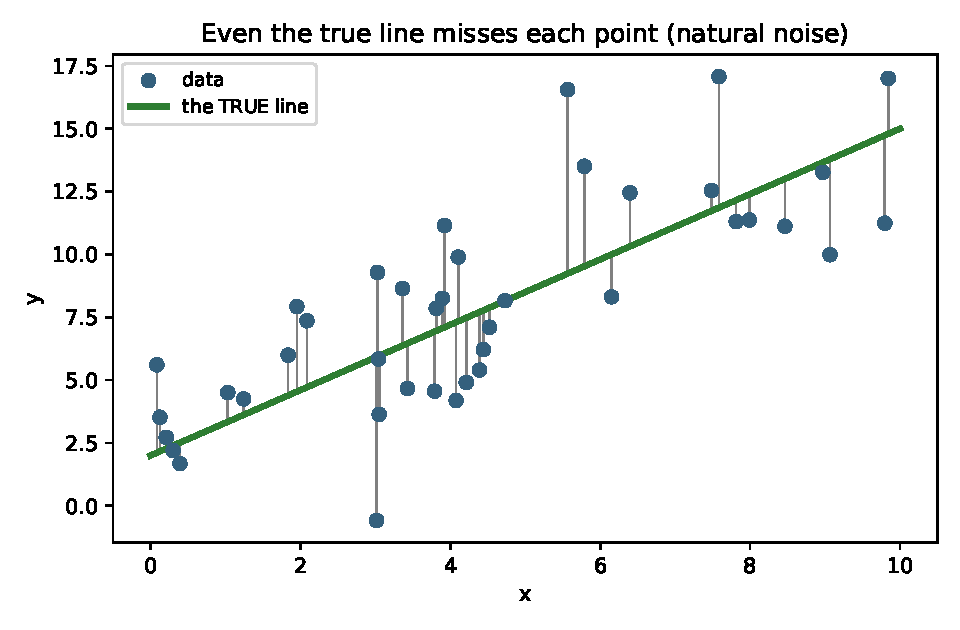
\includegraphics[width=\textwidth]{fig_irreducible.pdf}
\end{column}
\begin{column}{0.44\textwidth}
\small
Even if you \emph{knew} the true line exactly, individual points still scatter around it.
\begin{itemize}
  \item This is the noise you can never remove.
  \item It sets a hard floor on how accurate any prediction of a single case can be.
\end{itemize}
More data does \textbf{not} shrink this layer.
\end{column}
\end{columns}
\end{frame}

\begin{frame}{Layer 2: estimation uncertainty}
\begin{columns}[c]
\begin{column}{0.56\textwidth}
\centering
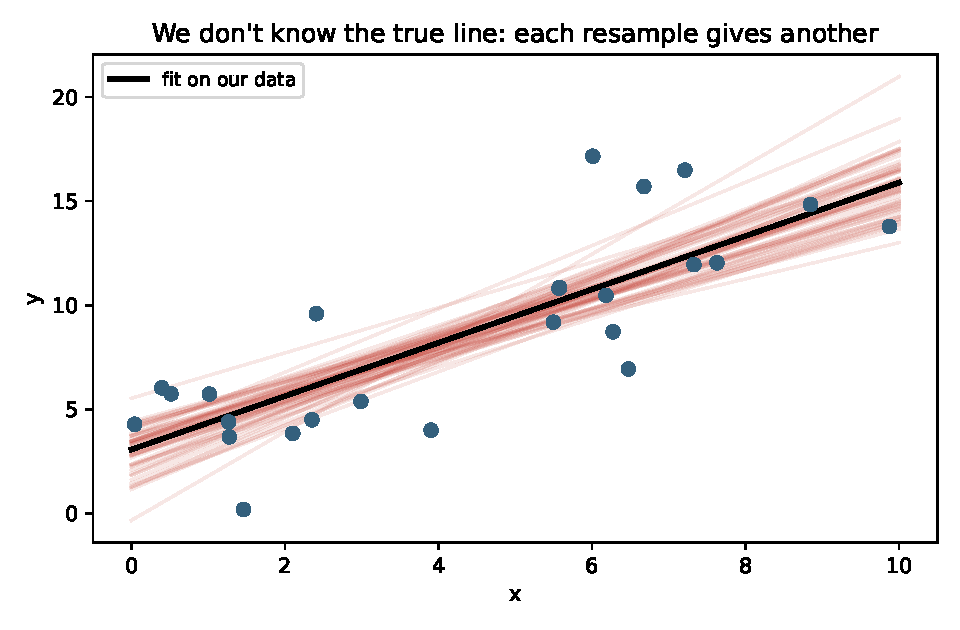
\includegraphics[width=\textwidth]{fig_ensemble.pdf}
\end{column}
\begin{column}{0.44\textwidth}
\small
We never see the true line. We estimate it from a finite sample, and a different sample would
give a slightly different line.
\begin{itemize}
  \item Each faint red line is a fit from a resample of the data.
  \item Their spread is the uncertainty in the line itself.
\end{itemize}
This layer \textbf{does} shrink as $n$ grows.
\end{column}
\end{columns}
\end{frame}

\begin{frame}{Layer 3: model (structural) error}
\begin{itemize}
  \item Maybe the truth is curved and we fit a line, or we left out a variable that matters.
  \item Then the model is \textbf{biased}: wrong in a systematic direction, not just noisy.
  \item Unlike estimation uncertainty, this does \alert{not} go away with more data. A bigger
        sample of the wrong model just nails down the wrong answer more precisely.
\end{itemize}
\begin{principle}{the layer that hides}
Noise and estimation error show up in the standard errors. Model error does not, because the
software reports tight intervals around a biased prediction without complaint.
\end{principle}
\end{frame}

\begin{frame}{Layer 4: distribution shift}
\begin{itemize}
  \item Every model assumes the future is drawn from the same world as the training data.
  \item When that breaks (a new market, a new season, a pandemic, a changed competitor) the
        model can fail even though nothing about the math is wrong.
  \item This is the layer that wrecks real production systems most often, and no in-sample
        statistic can warn you about it.
\end{itemize}
\begin{practice}{a classic}
``The model was 95\% accurate in testing and tanked in production.'' Usually the answer is
distribution shift or leakage, not a coding bug.
\end{practice}
\end{frame}

\begin{frame}{Putting it together: prediction band vs confidence band}
\begin{columns}[c]
\begin{column}{0.58\textwidth}
\centering
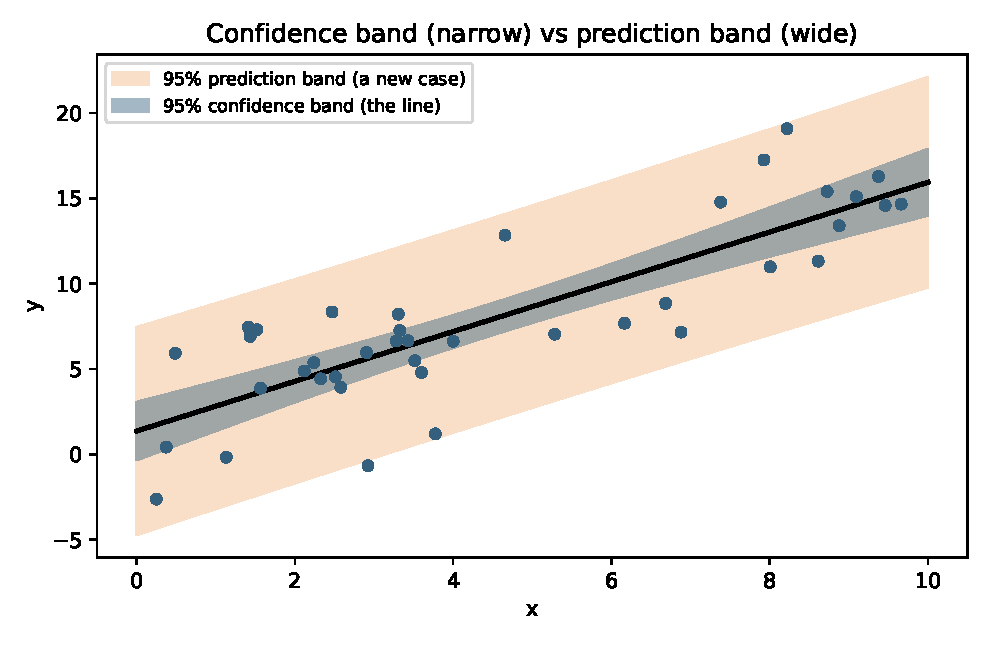
\includegraphics[width=\textwidth]{fig_bands.pdf}
\end{column}
\begin{column}{0.42\textwidth}
\small
\begin{itemize}
  \item The \textbf{confidence band} covers the \emph{line} (estimation only). Narrow.
  \item The \textbf{prediction band} covers a \emph{new case}, so it adds the irreducible
        noise. Much wider.
\end{itemize}
Here the prediction band is about \textbf{six times wider} than the confidence band. Predicting
a person is far harder than locating the average.
\end{column}
\end{columns}
\end{frame}

\begin{frame}{Your turn \#1}
\begin{yourturn}{which layer dominates?}
You're asked to predict \textbf{first-year sales of a brand-new product in a country you've
never sold in}.
\vspace{0.3em}

Turn to a neighbor: of the four layers (noise, estimation, model error, distribution shift),
which one worries you most here, and why?
\end{yourturn}
\end{frame}

\begin{frame}{Your turn \#1: answer}
\begin{itemize}
  \item \textbf{Distribution shift} and \textbf{model error} dominate: a new country and a new
        product are exactly the case your data does not cover.
  \item Estimation uncertainty (more data) and irreducible noise are real but secondary, and
        collecting more of the \emph{old} data won't help.
\end{itemize}
\begin{principle}{the diagnosis changes the cure}
If estimation is the problem, gather more data. If model error or shift is the problem, more of
the same data is useless. You need a different model, new data, or a humble, very wide interval.
\end{principle}
\end{frame}

% ======================================================================
\section{Estimating it}
% ======================================================================
\begin{frame}{How to get honest error bars}
\begin{itemize}
  \item \textbf{Prediction intervals} bundle the noise and estimation layers into one range for
        a new case.
  \item \textbf{The bootstrap or an ensemble} (refit on many resamples) shows the estimation
        and model wobble directly, as the spread of predictions.
  \item \textbf{Held-out residuals} are the most honest check: how big were the errors on data
        the model never saw? That spread is your real uncertainty.
\end{itemize}
\begin{principle}{trust the errors you actually made}
The most reliable error bar is empirical: look at how wrong the model was on fresh data, rather than
at the interval the formula prints from the training set.
\end{principle}
\end{frame}

\begin{frame}{Building a prediction interval from your own errors}
The most reliable interval needs no distributional theory at all:
\begin{enumerate}
  \item Fit the model on training data.
  \item Predict on a \textbf{held-out} set and collect the residuals
        $e_i = y_i - \hat y_i$.
  \item For a new case, report $\hat y \pm$ the 5th and 95th \emph{percentiles} of those held-out
        residuals.
\end{enumerate}
\begin{itemize}
  \item Worked: a model predicts 640 rentals. Held-out residuals run from $-210$ to $+260$ at the
        5th and 95th percentiles. Report \textbf{640, with a 90\% range of 430 to 900}.
  \item The interval is automatically the right width, because it is made of mistakes the model
        actually made.
\end{itemize}
\begin{principle}{why this beats the textbook formula}
The formula assumes the model is correct and the noise is constant. Held-out residuals assume
neither. They record what went wrong last time.
\end{principle}
\end{frame}

\begin{frame}{Your turn \#2}
\begin{yourturn}{which interval does the question need?}
Your model predicts revenue for a single store next month.
\begin{enumerate}
  \item The CFO asks: ``what will \emph{this store} bring in?''
  \item The board asks: ``what is average monthly revenue \emph{per store} across our 400
        stores?''
\end{enumerate}
With a neighbor: which question needs the wider interval, roughly how much wider, and why?
\end{yourturn}
\end{frame}

\begin{frame}{Your turn \#2: answer}
\begin{itemize}
  \item (1) needs a \textbf{prediction interval}: it carries the store's own irreducible
        variability plus our uncertainty about the model.
  \item (2) needs a \textbf{confidence interval} for the mean, which shrinks like $1/\sqrt{400}$
        and can be dramatically narrower.
  \item The prediction interval can easily be ten times wider. Handing the CFO the board's
        interval is the single most common way analysts get blamed for a ``wrong'' forecast.
\end{itemize}
\begin{principle}{one question to ask first}
Am I predicting \emph{one case} or locating \emph{an average}? Everything about the width follows
from that.
\end{principle}
\end{frame}

\begin{frame}{Calibration: do your intervals mean what they say?}
\begin{itemize}
  \item A 90\% interval is only honest if, across many predictions, the truth lands inside about
        \textbf{90\%} of the time.
  \item You can check this on held-out data: count the coverage. If your ``90\%'' intervals
        catch the truth 60\% of the time, they are too narrow, just like the calibration game.
\end{itemize}
\begin{trap}{confident and wrong}
An overconfident model is worse than an honest one. Narrow intervals feel impressive in a
meeting and cause disasters in production. Calibrated beats confident.
\end{trap}
\end{frame}

% ======================================================================
\section{Prediction follies}
% ======================================================================
\begin{frame}{Folly 1: extrapolation}
\begin{columns}[c]
\begin{column}{0.58\textwidth}
\centering
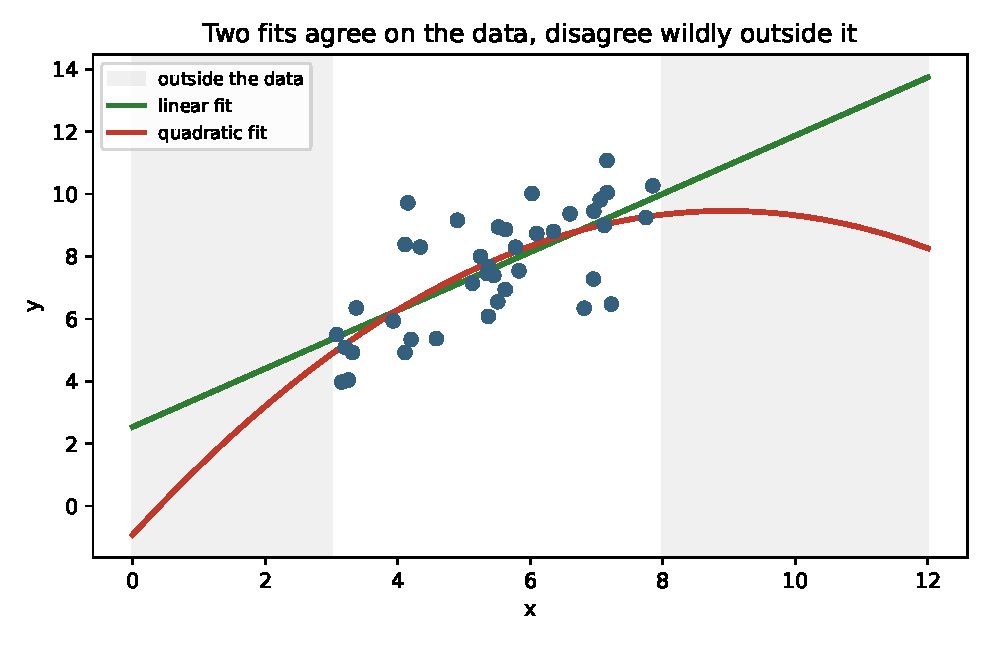
\includegraphics[width=\textwidth]{fig_extrapolation.pdf}
\end{column}
\begin{column}{0.42\textwidth}
\small
Two models can fit the data equally well and then \textbf{disagree wildly} once you leave the
range you observed.
\vspace{0.4em}

Mark Twain made the joke: extend the shrinking of the Mississippi River backward and ``a
million years ago'' it was over a million miles long. ``Wholesale returns of conjecture out of
a trifling investment of fact.''
\end{column}
\end{columns}
\end{frame}

\begin{frame}{Folly 2: regression to the mean}
\begin{columns}[c]
\begin{column}{0.58\textwidth}
\centering
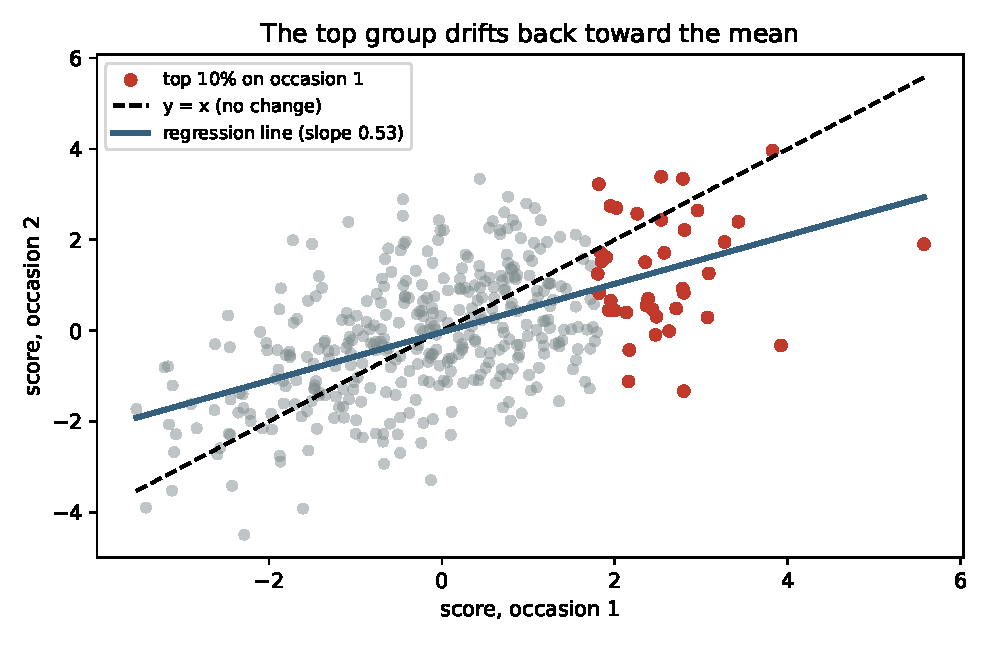
\includegraphics[width=\textwidth]{fig_regression_mean.pdf}
\end{column}
\begin{column}{0.42\textwidth}
\small
The top 10\% on occasion 1 averaged \textbf{2.55}. Next time they averaged \textbf{1.29}, with
\emph{no} change in true ability.
\begin{itemize}
  \item Extreme results are part skill, part luck, and luck doesn't repeat.
  \item This is the ``sophomore slump'' and the ``cover jinx.''
\end{itemize}
\end{column}
\end{columns}
\end{frame}

\begin{frame}{Folly 3: distribution shift, and a few more}
\begin{itemize}
  \item \textbf{Distribution shift:} a model trained on last year predicts this year badly,
        because the world moved.
  \item \textbf{Leakage:} a feature secretly contains the answer (or the future), so the model
        looks perfect in testing and useless in real life.
  \item \textbf{Goodhart's law:} once a predicted metric becomes a target, people game it and
        the prediction stops meaning anything.
\end{itemize}
\begin{trap}{too good to be true usually is}
A model that predicts almost perfectly is more often a sign of leakage than of genius. Your
first reaction to amazing accuracy should be suspicion, not celebration.
\end{trap}
\end{frame}

\begin{frame}{Scenario: the salesperson who ``slumped''}
\textbf{Setup.} Your top-performing rep last quarter had a much weaker second quarter. A manager
says the bonus program ruined their motivation.
\begin{itemize}
  \item Top performers are partly lucky, and luck doesn't repeat. A drop toward average is
        exactly what regression to the mean predicts, with no cause at all.
  \item The same logic flatters the bottom group: ``the training fixed our worst reps,'' when
        they would have bounced back anyway.
\end{itemize}
\begin{interview}{how to answer}
``Before blaming the bonus, I'd check whether this is just regression to the mean. To find a
real effect I'd compare against a control group, not against the same people's lucky quarter.''
\end{interview}
\end{frame}

% ======================================================================
\section{LLM check}
% ======================================================================
\begin{frame}{LLM check: mistake or not? (1 of 2)}
\begin{llmcheck}{we asked an LLM for a forecast}
\textbf{We told it:} ``Our model predicts \$420k for this house. Give me a 95\% interval.''\\[4pt]
\textbf{It answered:} ``95\% confident the price is \$420k plus or minus \$2k, so \$418k to
\$422k.''
\end{llmcheck}
\vspace{0.2em}
\centering\small Mistake, or no mistake?
\onslide<2->{%
\begin{trap}{verdict: mistake}
That \$2k is a confidence band on the \emph{average} house at those features. A single house
also carries irreducible noise, so the honest \emph{prediction} interval is far wider, more like
\$360k to \$480k. Quoting the CI as if it were the PI is dangerously overconfident.
\end{trap}}
\end{frame}

\begin{frame}{LLM check: mistake or not? (2 of 2)}
\begin{llmcheck}{same idea, a different answer}
\textbf{We told it:} ``We trained on 2019 data. Predict 2024 demand and tell me how much to
trust it.''\\[4pt]
\textbf{It answered:} ``The point forecast is X, but treat it cautiously: 2024 may differ from
2019 (distribution shift), so I'd widen the interval and validate on recent data before
relying on it.''
\end{llmcheck}
\vspace{0.2em}
\centering\small Mistake, or no mistake?
\onslide<2->{%
\begin{principle}{verdict: no mistake}
This is the careful answer: it flags distribution shift, refuses to over-trust the point, and
asks for recent validation. Exactly the instinct this module is building.
\end{principle}}
\end{frame}

% ======================================================================
\section{Workflow}
% ======================================================================
\begin{frame}{The arc of a prediction analysis}
The order still matters more than the syntax:
\begin{enumerate}
  \item \textbf{Name the target and the decision.} What are we predicting, and what will
        someone do with it?
  \item \textbf{Build and check on held-out data}, never on the training fit.
  \item \textbf{Attach an honest interval}, sized from real out-of-sample errors, not the
        training formula.
  \item \textbf{Check calibration and shift:} do the intervals cover at the rate they claim, and
        is the future like the past?
  \item \textbf{Communicate the uncertainty}, including extrapolation and ``this could be very
        wrong if the world changes.''
\end{enumerate}
\end{frame}

% ======================================================================
\section{Consolidate}
% ======================================================================
\begin{frame}{Producing a prediction with honest error bars}
\small
\begin{enumerate}
  \item \textbf{Name the target and the decision.} What will someone do with this number?
  \item \textbf{Fit on training data, predict on held-out data}, and keep those residuals.
  \item \textbf{Take the 5th and 95th percentiles of the held-out residuals} and attach them to the point prediction.
  \item \textbf{Check coverage} on data used for neither fitting nor calibration: do the 90\% intervals catch 90\%?
  \item \textbf{Ask which layer dominates}: noise, estimation, model structure, or shift.
  \item \textbf{Check whether you are extrapolating} past the range of the training data.
  \item \textbf{Report the point, the interval, and one sentence on when it stops being valid.}
\end{enumerate}
\end{frame}

\begin{frame}{The traps, all in one place}
\begin{trap}{the ones that bite most often}
\begin{itemize}
  \item Reporting a point prediction with no interval.
  \item Intervals that are too narrow (overconfidence).
  \item Quoting a confidence interval when you needed a prediction interval.
  \item Extrapolating past the range of the data.
  \item Assuming the future matches the training data.
  \item Mistaking regression to the mean for a real effect.
  \item Trusting amazing accuracy without checking for leakage.
\end{itemize}
\end{trap}
\end{frame}

\begin{frame}{Ten questions to be able to answer}
\begin{enumerate}\small
  \item A prediction is wrong. Walk me through the possible sources of the error.
  \item What is the difference between irreducible noise and estimation uncertainty?
  \item Which sources of error shrink with more data, and which do not?
  \item Confidence interval or prediction interval: which do you give a customer, and why?
  \item How would you actually put honest error bars on a forecast?
  \item Your model was great in testing and failed in production. What happened?
  \item Your best performer slumped the next quarter. Did your intervention fail?
  \item A model predicts almost perfectly. Are you excited or suspicious?
  \item Why is extrapolating beyond the data so dangerous?
  \item What does it mean for intervals to be calibrated, and how would you check?
\end{enumerate}
\end{frame}

\begin{frame}{Mastery checklist}
You have this unit when you can, from memory:
\begin{itemize}
  \item report a prediction as a point plus an honest interval
  \item name the four layers of error and say which shrink with data
  \item explain why a prediction interval is wider than a confidence interval
  \item estimate uncertainty from held-out errors and the bootstrap
  \item recognize extrapolation, regression to the mean, leakage, and shift
  \item explain what calibration is and how to check it
\end{itemize}
\end{frame}

\begin{frame}{How to report a prediction}
\begin{principle}{the reusable structure}
\begin{enumerate}
  \item \textbf{The point:} the model's best guess.
  \item \textbf{The interval:} honest, sized from real out-of-sample errors.
  \item \textbf{The sources:} which layer dominates the uncertainty here?
  \item \textbf{The boundaries:} are we extrapolating, and could the world have shifted?
  \item \textbf{The caveat:} one sentence on when this prediction should not be trusted.
\end{enumerate}
\end{principle}
\centering
A point with no range is a guess. A point with an honest range is a forecast.
\end{frame}

\begin{frame}{What you should be able to do with software}
\small
Nobody is asking you to memorize syntax. You are expected to know \emph{which} procedure the
question calls for, what to hand it, and what the output means. With an AI assistant open, you
should be able to produce any of these and defend the result.
\begin{center}\footnotesize
\begin{tabular}{p{0.44\textwidth} p{0.46\textwidth}}
\toprule
\textbf{You should be able to} & \textbf{What you would reach for} \\
\midrule
Predictions from a fitted model & \texttt{model.predict(X\_new)} \\
Held-out residuals & \texttt{y\_test - model.predict(X\_test)} \\
An empirical prediction interval & \texttt{np.percentile(resid, [5, 95])} \\
Confidence versus prediction band in OLS & \texttt{fit.get\_prediction(X)} \newline \texttt{\ \ .conf\_int(obs=True)} \\
Coverage check & count how often the truth lands inside \\
Estimation wobble via resampling & refit on bootstrap samples and spread the predictions \\
Turn a predictive distribution into a decision & simulate outcomes, then average the cost \\
\bottomrule
\end{tabular}
\end{center}
\vspace{0.2em}
\centering\small
If you cannot say what the output means, the fact that you produced it is worth nothing.
\end{frame}

\begin{frame}{Where we go next}
\begin{itemize}
  \item So far the prediction has been a number. \textbf{Unit 8} turns to categorical outcomes:
        rates, tables, and predicting a yes or no, where the model outputs a probability and
        somebody has to choose a threshold.
  \item The same ideas carry over: a probability is a prediction with uncertainty, it can be
        miscalibrated, and the \emph{cost} of being wrong is rarely the same in both directions.
\end{itemize}
\begin{principle}{the through-line}
Whether the output is a number or a yes/no, the job is the same: give your best guess, say how
sure you are, and know when not to trust it.
\end{principle}
\end{frame}

\end{document}
